\chapter{Introduction}
\label{chp:introduction}
The widespread usage of GPS receivers, including personal devices and objects such as mobile phones, vehicles, and
wearable devices, are generating massive spatio-temporal datasets. Such datasets can contain information that range from
the daily routine of residents of a city~\citep{whatdidyoudo} to behaviors of wild animals in a specific region
\citep{trajclustering}\citep{miningperiodic}. Given that most recent datasets have a number of features, one can
use them to extract patterns to answer questions such as "What are the busiest times and locations of a city?"
\citep{smartcities}\citep{visualtrafficjam}, "What is the movement behavior of wild animals in their habitat?"
\citep{movemine}, and the like.

In the aforementioned examples, some of the  queries are intrinsically related to collaborative or group patterns, such
as flock \citep{gudefficient}, convoy \citep{convoy}, swarm \citep{swarm}, and the like. Those patterns
contain moving objects that have a strong relationship by being close to each other, within a certain distance range and
during some minimum time interval. Due to the wide range of applicability in the real world (e.g. city roads planning,
intelligent transportation, and wildlife conservation), the data mining of such patterns has gained great importance in
both industry and academy. There are a number of research challenges in this topic, specially regarding the development
of accurate algorithms to detect those patterns. In addition of being precise, it is of paramount importance to design
fast algorithms so that they can be keep up with real-time data. Hence, efficiently extraction of data patterns for
real-time analysis and on the fly decision-making is still an open challenge.

A seminal formal definition of the flock pattern was proposed by \citep{remo} and \citep{gudefficient} and since
then, a myriad of other studies has follow suit (we refer the reader to Section~\ref{sec:related} for some of them),
mainly due to the interests in developing mechanisms to solve real-world problems in the scope of Internet of Things
(IoT) \citep{iot} and Smart Cities \citep{smartcities}. According to \citep{gudefficient}, a flock pattern
consists of a minimum number of entities that are within a disk of radius \textit{r} at a given time. However, this
definition only applies to one single time step and does not help on extracting some useful collective behavior
information. Such initial definition was then extended by \citep{gudreportingflock}, introducing the minimum time
interval $\delta$ that the entities should stay together in order to characterize a flock pattern, as depicted by Fig.
\ref{fig:flocks}. The figure shows a flock pattern that lasts three time steps and is formed by trajectories $T_1$,
$T_2$ and $T_3$. Trajectories $T_4$ and $T_5$ do not form a flock because there are no disks enclosing them in all three
time steps.

\begin{figure}
    \centering
    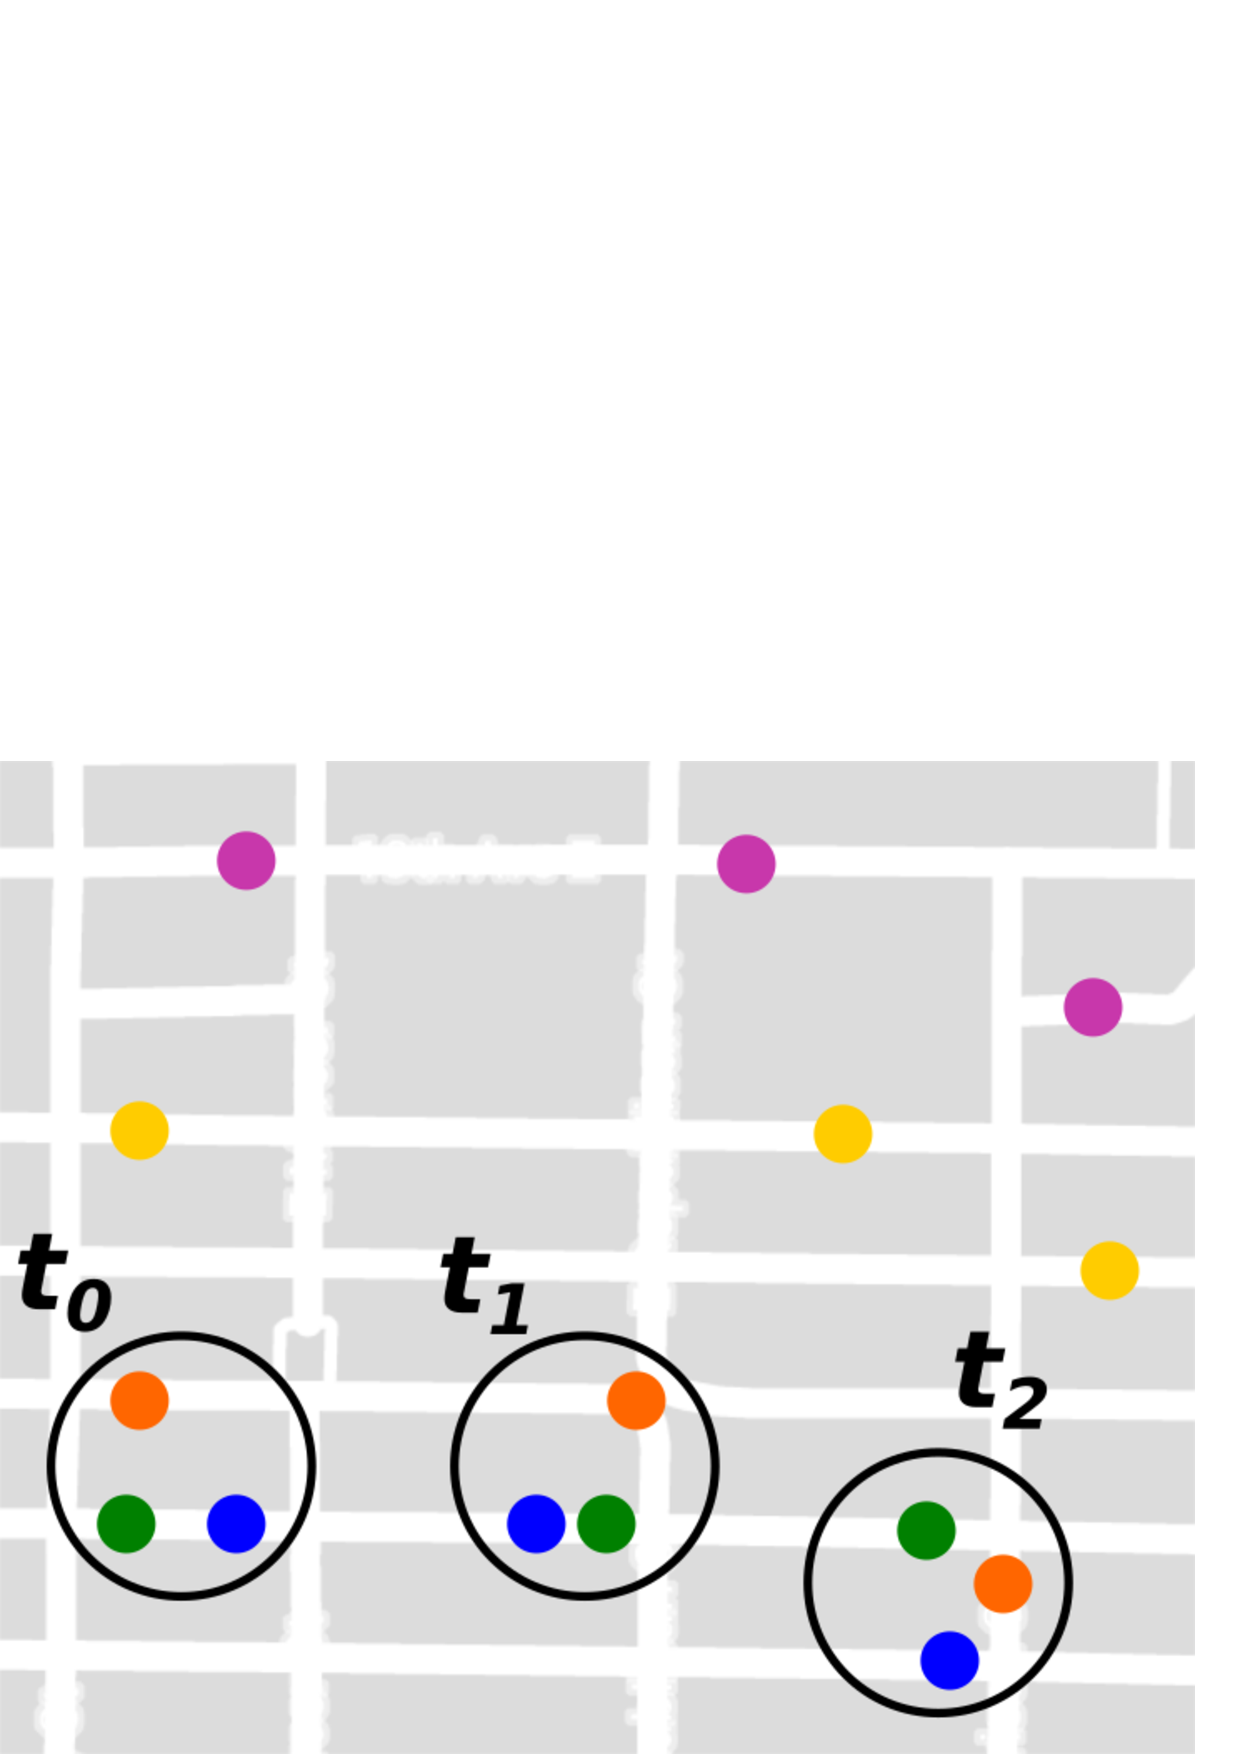
\includegraphics[width=0.7\linewidth]{images/flock_pattern.png}
    \caption{T1, T2 and T3 form a flock of size 3 with minimum length of three time steps, with a disk enclosing all
        trajectories at each time step (\hspace{-0.005cm}\citep{vieira})}
    \label{fig:flocks}
\end{figure}

One major problem on detecting flock patterns accurately is to find the disks that enclose the trajectories in each time
step. Since the disks centers do not need to match any point in the dataset, there can be infinite disks. Vieira et al.
\citep{vieira} proposed a way to limit the number of disks to generate and analyze, so a finite number of disks are
in place to cluster the trajectories in those disks. He also proposed an algorithm to find the flock pattern, namely
Basic Flock Evaluation (BFE). Such algorithm suffers from some severe performance limitations, which we discuss more in
Section~\ref{sec:related} and \ref{sec:algorithm}.

This paper proposes an efficient flock detection algorithm aiming at achieving considerable gains in execution time,
without compromising accuracy, thus targeting real-time deployment and online processing. Our target scenarios are the
ones related to Smart Cities, where decisions need to be made on the fly
\citep{ieeesmartcities}\citep{springersmartcities}. Such gains are made possible by creating a filtering
heuristic, based on bitmaps, in order to save processing time. Our proposal focuses on identifying objects that can
actually form a flock, resulting in a huge reduction in the number of disks generated. Our results indicate that our
proposal outperforms the current state-of-the-art techniques, by achieving 99\% CPU time improvement and 96\% disks
generation reduction in some relevant scenarios.

The remainder of the paper is organized as follows: Section~\ref{sec:related} highlights the related work in both flock
detection and trajectory data mining and Section~\ref{sec:concepts} presents the technical background necessary to
understand this paper. It also describes the baseline algorithm. Section~\ref{sec:algorithm} proposes our algorithm,
called \textbf{Bit}maps for \textbf{D}isk \textbf{F}iltering (BitDF), whereas Section~\ref{sec:results} shows the
results we obtained in our experiments. We draw some concluding remarks and provide directions for future work in
Section~\ref{sec:conclusion}.
